\subsection{Algorytm \textit{przeszukiwania w głąb}}

\textbf{Algorytm przeszukiwania w głąb} (ang. \textit{Depth-First Search}, DFS)~\cite{cormen2009} to klasyczna metoda eksploracji grafu, która w kontekście generowania labiryntu pozwala na systematyczne zagłębianie się w kolejne, jeszcze nieodwiedzone komórki planszy z wykorzystaniem mechanizmu rekurencji. Algorytm rozpoczyna od wybranej komórki startowej i rekursywnie odwiedza sąsiadujące, nieodwiedzone komórki, usuwając ściany między nimi w celu utworzenia ścieżek. Algorytm działa w następujący sposób:

\begin{enumerate}
    \item Na początku algorytmu, tworzony jest labirynt, którego wszystkie pola stanowią ściany. Rysunek \ref{fig:dfs_gen_step_1} przedstawia początkowy układ labiryntu.
    
    \begin{figure}[H]
    \centering
    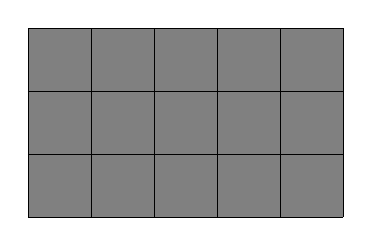
\begin{tikzpicture}[scale=0.8]
        \foreach \x in {0,...,4} {
            \foreach \y in {0,...,2} {
                \fill[gray] (\x,\y) rectangle ++(1,1);
            }
        }
        \draw[step=1cm,ultra thin,black] (0,0) grid (5,3);
    \end{tikzpicture}
    \caption{\centering Cała plansza stanowi ściany.}
    \label{fig:dfs_gen_step_1}
\end{figure}

    \item W następnym kroku wybierana jest losowa komórka, która jest oznaczana jako przejście. Na rysunku \ref{fig:dfs_gen_step_2} pokzano losowo wybrane pole labiryntu.

    \begin{figure}[H]
    \centering
    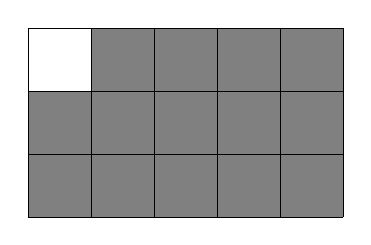
\begin{tikzpicture}[scale=0.8]
        \foreach \x in {0,...,4} {
            \foreach \y in {0,...,2} {
                \fill[gray] (\x,\y) rectangle ++(1,1);
            }
        }
        \fill[white] (0, 2) rectangle ++(1,1);
        \draw[step=1cm,ultra thin,black] (0,0) grid (5,3);
    \end{tikzpicture}
    \caption{\centering Losowo wybrane pole, zamienione na przejście.}
    \label{fig:dfs_gen_step_2}
\end{figure}

    \item Następnie algorytm losowo wybiera jedną z sąsiadujących komórek. Podobnie jak w~przypadku \textit{algorytmu Prima}, przyjęto, że komórka sąsiadująca to dowolna komórka oddalona o jedno pole w pionie lub poziomie. Podczas ruchu przejścia są weryfikowane - mogą bowiem znajdować się poza granicami planszy. Rysunek~\ref{fig:dfs_gen_step_3} przedstawia taką sytuację.
    
    \begin{figure}[H]
    \centering
    \begin{tikzpicture}[scale=0.8]
        \foreach \x in {0,...,4} {
            \foreach \y in {0,...,2} {
                \fill[gray] (\x,\y) rectangle ++(1,1);
            }
        }
        \fill[white] (0, 2) rectangle ++(1,1);

        \fill[white] (0,0) rectangle ++(1,1);
        \fill[pattern=north east lines, pattern color=black] (0,0) rectangle ++(1,1);

        \fill[white] (2,2) rectangle ++(1,1);
        \fill[pattern=north east lines, pattern color=black] (2,2) rectangle ++(1,1);

        \draw[->, very thick, black] (0.5,2.5) -- (2.5,2.5);
        \draw[->, very thick, black] (0.5,2.5) -- (0.5,0.5);
        \draw[->, very thick, black] (0.5,2.5) -- (0.5,4.5);
        \draw[->, very thick, black] (0.5,2.5) -- (-1.5,2.5);

        \draw[dashed] (-2,2) rectangle ++(1,1);
        \draw[dashed] (0,4) rectangle ++(1,1);

        \draw (0.5,2.5) circle[radius=4mm];

        \draw[step=1cm,ultra thin,black] (0,0) grid (5,3);
    \end{tikzpicture}
    \caption{\centering Potencjalne dalsze ruchy algorytmu (oznaczone strzałkami). Nieistniejące pola (poza labiryntem) oznaczono przerywaną linią, natomiast pola stanowiące rzeczywiste możliwe przejścia zakreskowano. Aktualnie rozpatrywaną komórkę oznaczono kółkiem.}
    \label{fig:dfs_gen_step_3}
\end{figure}

    \item Po losowym wybraniu nowej komórki do której można utworzyć ścieżkę, algorytm usuwa ścianę dzielącą ją od poprzedniej i kontynuuje działanie na tej komórce. Warto jednak zauważyć, że ze względu na rekurencyjny charakter algorytmu, poprzednie możliwe ruchy są zapisywane na \textit{stosie}. Oznacza to, że algorytm generuje labirynt \textit{w~głąb}, podejmując decyzję o kontynuacji na podstawie pierwszej dostępnej komórki, a dopiero w przypadku braku dalszych możliwości następuje wycofanie do wcześniejszego kroku. Rysunek~\ref{fig:dfs_gen_step_4} ilustruje cały ten proces.

    \begin{figure}[H]
    \centering
    \begin{tikzpicture}[scale=0.8]
        \foreach \x in {0,...,4} {
            \foreach \y in {0,...,2} {
                \fill[gray] (\x,\y) rectangle ++(1,1);
            }
        }
        \fill[white] (0, 2) rectangle ++(1,1);
        \fill[white] (1, 2) rectangle ++(1,1);
        \fill[white] (2, 2) rectangle ++(1,1);

        \fill[white] (0,0) rectangle ++(1,1);
        \fill[pattern=north east lines, pattern color=black] (0,0) rectangle ++(1,1);

        \fill[white] (2,0) rectangle ++(1,1);
        \fill[pattern=north east lines, pattern color=black] (2,0) rectangle ++(1,1);

        \draw[->, very thick, black, dashed] (0.5,2.4) -- (0.5,0.5);

        \draw[->, very thick, black] (2.5,2.5) -- (4.5,2.5);
        \draw[->, very thick, black] (2.5,2.5) -- (2.5,0.5);
        \draw[->, very thick, black] (2.5,2.5) -- (2.5,4.5);
        \draw[->, very thick, black] (2.5,2.5) -- (0.6,2.5);

        \draw[dashed] (2,4) rectangle ++(1,1);

        \draw (2.5,2.5) circle[radius=4mm];

        \draw[step=1cm,ultra thin,black] (0,0) grid (5,3);
    \end{tikzpicture}
    \caption{\centering Wybór kolejnego pola. Ruchy występujące w poprzednich krokach, ale nie brane pod uwagę w bieżącej iteracji oznaczono przerywaną linią.}
    \label{fig:dfs_gen_step_4}
\end{figure}

    \begin{figure}[H]
    \centering
    \begin{tikzpicture}[scale=0.8]
        \foreach \x in {0,...,4} {
            \foreach \y in {0,...,2} {
                \fill[gray] (\x,\y) rectangle ++(1,1);
            }
        }
        \fill[white] (0, 2) rectangle ++(1,1);
        \fill[white] (1, 2) rectangle ++(1,1);
        \fill[white] (2, 2) rectangle ++(1,1);

        \fill[white] (0,0) rectangle ++(1,1);
        \fill[pattern=north east lines, pattern color=black] (0,0) rectangle ++(1,1);

        \fill[white] (2,0) rectangle ++(1,1);
        \fill[white] (2,1) rectangle ++(1,1);
        \fill[white] (3,0) rectangle ++(1,1);
        \fill[white] (4,0) rectangle ++(1,1);
        \fill[white] (4,1) rectangle ++(1,1);
        \fill[white] (4,2) rectangle ++(1,1);

        \draw[->, very thick, black, dashed] (2.5,0.6) -- (2.5,2.4);
        \draw[->, very thick, black, dashed] (2.4,0.5) -- (0.6,0.5);

        \draw[->, very thick, black, dashed] (4.4,0.5) -- (2.6,0.5);

        \draw[->, very thick, black, dashed] (0.5,2.4) -- (0.5,0.6);

        \draw[->, very thick, black, dashed] (2.65,2.62) -- (4.32,2.62);
        \draw[->, very thick, dashed] (2.4,2.5) -- (0.6,2.5);

        \draw[->, very thick, dashed] (4.5,2.6) -- (4.5,4.4);
        \draw[->, very thick, dashed] (4.6,2.5) -- (6.4,2.5);
        \draw[->, very thick, black, dashed] (4.32,2.38) -- (2.65,2.38);
        \draw[->, very thick, dashed] (4.5,2.4) -- (4.5,0.6);

        \draw[dashed] (6,2) rectangle ++(1,1);
        \draw[dashed] (4,4) rectangle ++(1,1);

        \draw (4.5,2.5) circle[radius=4mm];

        \draw[step=1cm,ultra thin,black] (0,0) grid (5,3);
    \end{tikzpicture}
    \caption{\centering Stan labiryntu po kilku następnych iteracjach. Algorytm zacznie wracać, gdyż nie istnieje żaden prawidłowy ruch generujący przejście - ruchy w górę lub prawo spowodują wygenerowanie przejścia poza planszę, a ruchy w lewo bądź dół - powstanie pętli.}
    \label{fig:dfs_gen_step_5}
\end{figure}

    \begin{figure}[H]
    \centering
    \begin{tikzpicture}[scale=0.8]
        \foreach \x in {0,...,4} {
            \foreach \y in {0,...,2} {
                \fill[gray] (\x,\y) rectangle ++(1,1);
            }
        }
        \fill[white] (0, 2) rectangle ++(1,1);
        \fill[white] (1, 2) rectangle ++(1,1);
        \fill[white] (2, 2) rectangle ++(1,1);

        \fill[white] (0,0) rectangle ++(1,1);
        \fill[pattern=north east lines, pattern color=black] (0,0) rectangle ++(1,1);

        \fill[white] (2,0) rectangle ++(1,1);
        \fill[white] (2,1) rectangle ++(1,1);
        \fill[white] (3,0) rectangle ++(1,1);
        \fill[white] (4,0) rectangle ++(1,1);
        \fill[white] (4,1) rectangle ++(1,1);
        \fill[white] (4,2) rectangle ++(1,1);

        \draw[->, very thick, black, dashed] (2.5,0.6) -- (2.5,2.4);
        \draw[->, very thick, black, dashed] (2.4,0.5) -- (0.6,0.5);

        \draw[->, very thick, black, dashed] (0.5,2.4) -- (0.5,0.6);

        \draw[->, very thick, black, dashed] (2.65,2.5) -- (4.32,2.5);
        \draw[->, very thick, dashed] (2.4,2.5) -- (0.6,2.5);

        \draw (2.5,0.5) circle[radius=4mm];

        \draw[step=1cm,ultra thin,black] (0,0) grid (5,3);
    \end{tikzpicture}
    \caption{\centering Odnalezienie prawidłowego przejścia przy powrocie.}
    \label{fig:dfs_gen_step_6}
\end{figure}

    \input{sections/maze_generation/subsections/dfs_algorithm/figures/dfs_gen_step_7}

    \begin{figure}[H]
    \centering
    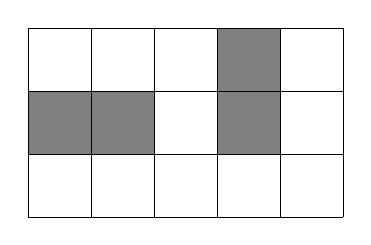
\begin{tikzpicture}[scale=0.8]
        \foreach \x in {0,...,4} {
            \foreach \y in {0,...,2} {
                \fill[gray] (\x,\y) rectangle ++(1,1);
            }
        }
        \fill[white] (0, 2) rectangle ++(1,1);
        \fill[white] (1, 2) rectangle ++(1,1);
        \fill[white] (2, 2) rectangle ++(1,1);

        \fill[white] (0,0) rectangle ++(1,1);
        \fill[white] (2,0) rectangle ++(1,1);
        \fill[white] (2,1) rectangle ++(1,1);
        \fill[white] (3,0) rectangle ++(1,1);
        \fill[white] (4,0) rectangle ++(1,1);
        \fill[white] (4,1) rectangle ++(1,1);
        \fill[white] (4,2) rectangle ++(1,1);
        \fill[white] (1,0) rectangle ++(1,1);

        \draw[step=1cm,ultra thin,black] (0,0) grid (5,3);
    \end{tikzpicture}
    \caption{\centering Końcowy wygląd labiryntu. Pozostałe powroty nie wygenerowały żadnych przejść ze względu na brak prawidłowych ruchów.}
    \label{fig:dfs_gen_step_8}
\end{figure}

\end{enumerate}

